\subsection{One dimensional hydrogen chain}
\label{subsection:1dhydrogen}
We now move on to one of the simplest extended \emph{ab initio} systems, a hydrogen chain in one dimension with periodic boundary conditions. The one-dimensional hydrogen chain has been used as a model for validating a variety of modern \textit{ab initio} many-body methods \cite{H10_Simons}. 
We consider the case of $10$ atoms with periodic boundary conditions and work in a regime where the inter-atomic distance $r$ is in the range $r=1.5$ to $3.0$ \AA, such that the system is  well described in terms of primarily $s$-like orbitals. 

For a given $r$, we first obtain single-particle Kohn-Sham orbitals from a set of spin-unrestricted and 
spin-restricted DFT-PBE calculations. The localized orbital basis upon which the RDMs (descriptors) 
are evaluated is obtained by generating intrinsic atomic orbitals (IAO) from the Kohn-Sham orbitals 
orthogonalized using the L\"owdin procedure (see Figure~\ref{fig:fit_quality}). These are the orbitals that enter the one-band Hubbard Hamiltonian. 
Then, to generate a database of wavefunctions needed for the DMD, we produce a set of Slater-Jastrow 
wavefunctions consisting of singles and doubles excitations to the Slater determinant:
\begin{subequations}
\begin{eqnarray}
| s \rangle = & e^J \Big[a^\dagger_{i \eta} a_{k \eta}   | KS \rangle \Big] \,,\\
| d \rangle = & \: e^J \Big[a^\dagger_{i \eta} a^\dagger_{j \eta'} a_{k \eta'} a_{l \eta}   | KS \rangle\Big] ,
\end{eqnarray}
\end{subequations}
where $|KS\rangle$ is the Slater determinant of occupied Kohn-Sham orbitals, $\eta$ and $\eta'$ are spin indices, \lucas{it is unclear here if $\eta$ and $\eta'$ are allowed to be different. }
and $a_{i}^\dagger$ ($a_{i}$) is a single-electron creation (destruction) operator corresponding to a particular Kohn-Sham orbital. $k,l$ refer to occupied orbitals in the original Slater determinant, while $i,j$ are virtual orbitals. 
$e^J$ is a Jastrow factor optimized by minimizing the variance of the local energy. 
We compute the energies (expectation values of the Hamiltonian) and the RDMs on all the wave functions within DMC. 
By computing the trace of the resulting 1-RDMs, we verify that all the electrons present in the system are represented within the localized basis of $s$-like orbitals. 
If the trace of the 1-RDM falls below the nominal number of electrons for a particular state,\lucas{be more specific. What are the thresholds?} it 
indicates that some higher-energy orbitals are occupied ($p$-like orbitals, in the case of hydrogen\lucas{could be 2s}), and that the state can not be described by the low-energy model Hamiltonian.\lucas{Are these very high energy states?}
 We exclude such states from the data set. 
The acquired data set is then used in DMD to downfold to a one-band Hubbard Hamiltonian.ab initio
\begin{figure}
\centering
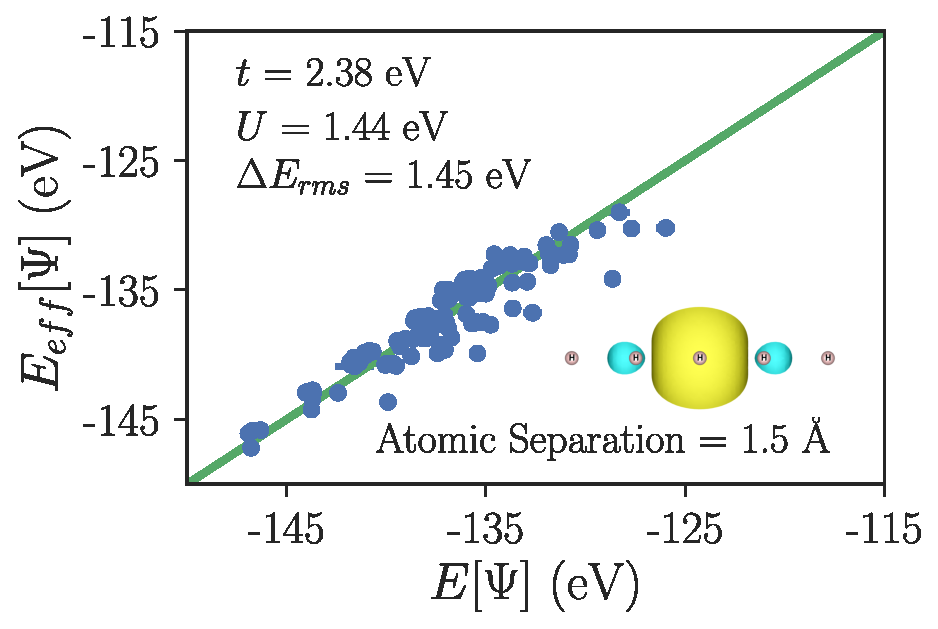
\includegraphics[scale=0.45]{{./Figures/H_chain_fit_model_length1.5_tUs_inset}.eps}
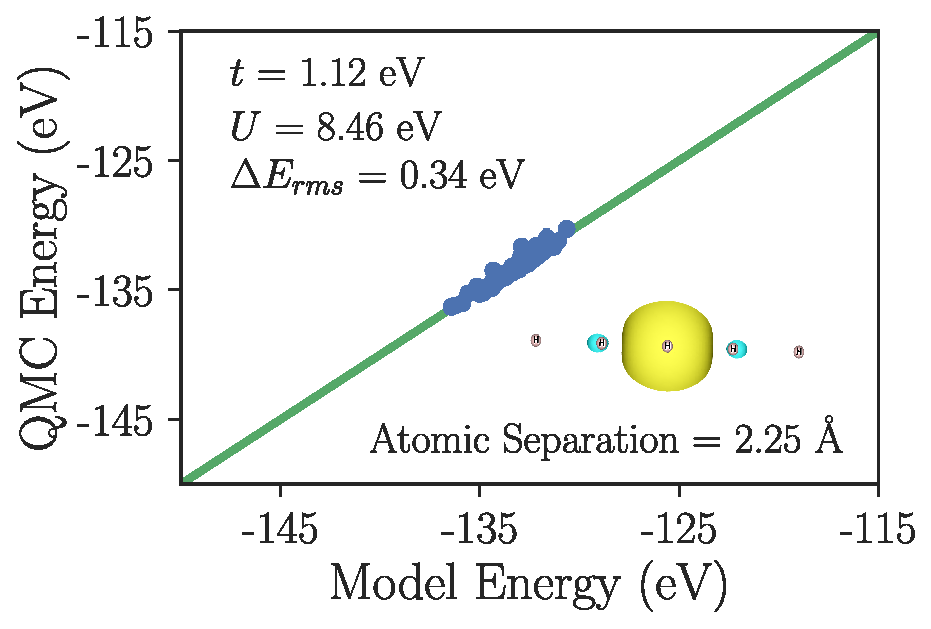
\includegraphics[scale=0.45]{{./Figures/H_chain_fit_model_length2.25_tUs_inset}.eps}
\caption{DMC energy versus the reconstructed 
model energy for the H$_{10}$ chain at (A) 1.5 \AA \: and (B) 2.25 \AA \:. The energy range of excitations 
narrows significantly for larger interatomic separation. Insets show the intrinsic atomic orbitals which constitute the one-body space 
which was used for calculating the reduced density matrices (descriptors).  
\lucas{Need A,B,C labels. $R^2$ should be in the next figure with other vs $r$ things}. 
\lucas{Should standardize these graphs as $E[\Psi]$ and $E_{eff}[\Psi]$}}
\label{fig:fit_quality}
\end{figure}

Figure~\ref{fig:fit_quality} shows our DMD fits for two representative $r$. 
The model energy is the energy reconstructed from the optimized parameters $t$ and $U$ and the RDMs. 
For $r=1.5$ \AA, there is considerable spread in the data from the 45 degree line indicating that the simple short range Hubbard model 
is insufficient for an \textit{accurate} description in the corresponding energy window. 
In contrast, the R$^2$ fit parameter is significantly larger for larger $r$, suggesting the increased 
effectiveness of the one-band Hubbard model, as seen in Figure~\ref{fig:Parameters-vs-Bond-t}(C).   \lucas{What is the conclusion of this paragraph?}

\begin{figure}
\centering
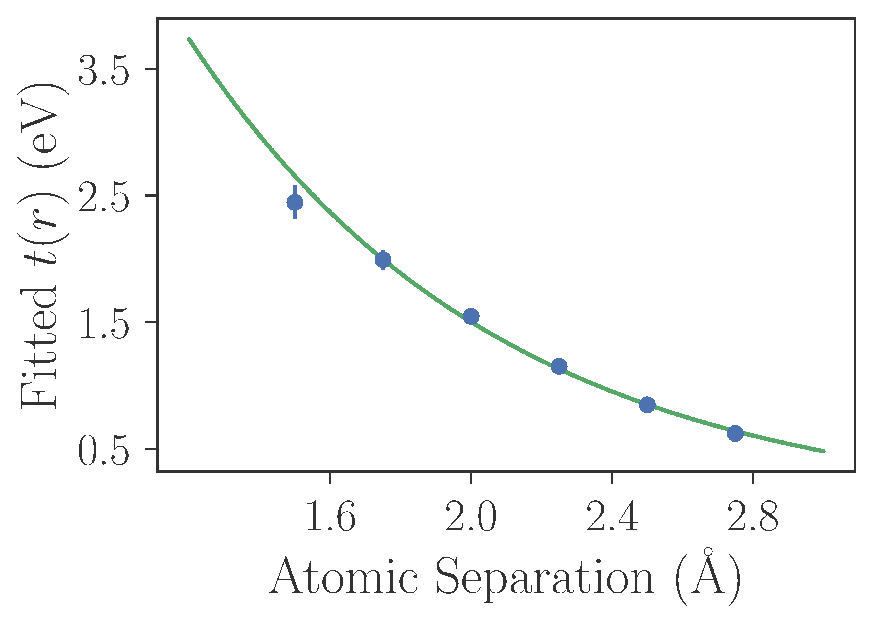
\includegraphics[scale=0.35]{./Figures/fitted_t_values_no_offset_h10_chain.eps}
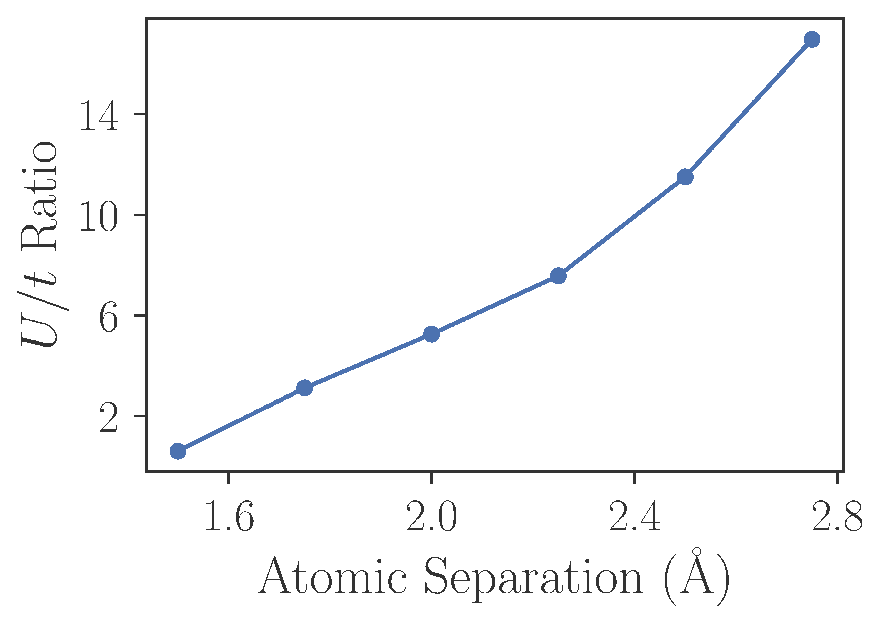
\includegraphics[scale=0.35]{./Figures/Ust_ratio_vs_separation_h_chain.eps}
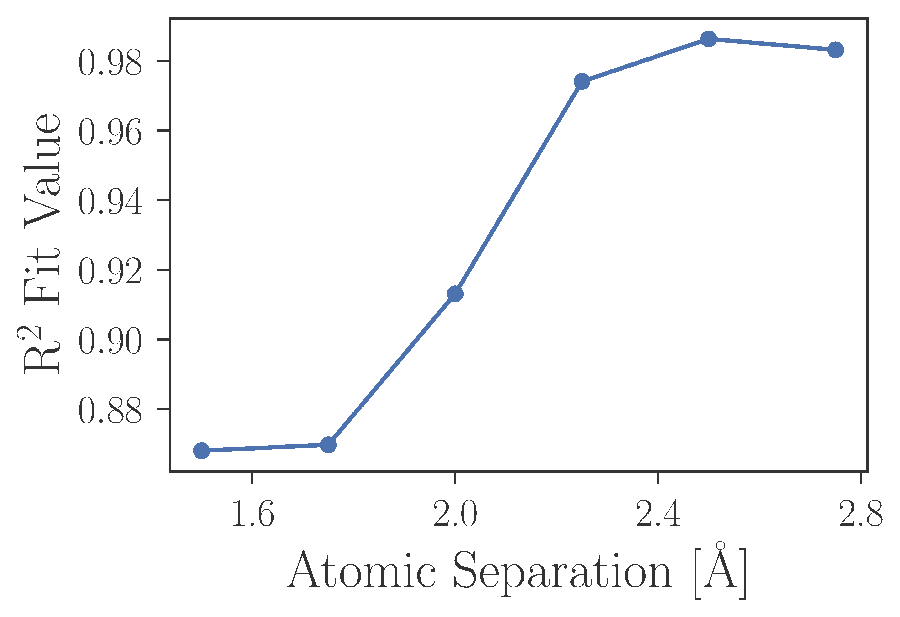
\includegraphics[scale=0.35]{{./Figures/r2_ut_vs_separation_h_chain}.eps}
\caption{(A) The one-body hopping $t$ parameter as a function of interatomic distance for the periodic H$_{10}$ chain, obtained from a fitted $U$-$t$ model. $t$ declines to zero as $r$ increases. (B) The ratio $U/t$ for the fitted parameter values as a function of interatomic separation. The ratio is small at lower bond-lengths, where $t$ is more relevant in describing the system, and larger at longer bond-lengths, where inter-site hopping is less significant. (C) The R$^2$ fit parameters obtained from fitting the $U$-$t$ model to the H$_{10}$ chain, as a function of interatomic separation. }\label{fig:Parameters-vs-Bond-t}
\end{figure}

Figure~\ref{fig:Parameters-vs-Bond-t} shows trends of the DMD values of $t$ and $U$ as a function of $r$. 
Consistent with physical intuition, $t$ decreases towards zero at larger $r$
and the value of $U/t$ rises. 


However, as previously mentioned, the single-band 
Hubbard model is not expected to describe the hydrogen chain well at small distances. 
The one dimensional Hubbard model with $U/t>0$ will always result in 
an Mott insulating state. In comparison, for the idealized hydrogen chain, the 
metal-to-insulator transition has been shown to occur at $r_c \sim 1.8$\AA~\cite{Stella2011}, which would correspond 
to a finite non-zero $U$. This indicates that at small distance, the higher energy orbitals play a nontrivial 
role in stabilizing the metallic state of hydrogen, instead of merely renormalizing the effective strength of $U$. 
At small distances, other interactions like nearest neighbor Coulomb 
and exchange interactions also become important for $r<r_c$ \cite{ZhengThesis}. The kink that appears near $r_c$ in the R$^2$ plot [Figure~\ref{fig:fit_quality}(C)] is a manifestation of underlying metal-to-insulator transition in the \textit{ab initio} system. 
\lucas{this paragraph does not have a clear point. Separate your ideas more. What are you trying to say?} 
